%!TEX program = xelatex
% Note: this template must be compiled with XeLaTeX rather than PDFLaTeX
% due to the custom fonts used. The line above should ensure this happens
% automatically, but if it doesn't, your LaTeX editor should have a simple toggle
% to switch to using XeLaTeX.

\documentclass[
	aspectratio=169, % Uncomment to use an aspect ratio of 16:9 (160 mm by 90 mm)
	%aspectratio=43, % Uncomment to use an aspect ratio of 4:3 (128mm by 96mm)
	t, % Top align all slide content by default
	onlytextwidth, % Typeset content in columns at text width
	10pt, % Default font size, use 10pt for the 16:9 aspect ratio and 8pt for the 4:3 aspect ratio
]{beamer}

\usepackage{../ImperialTheme/beamerthemeImperial} % Use the Imperial theme

\def\imagefolder{../ImperialTheme/Images/}

\title{Linear instabilities with the Incompressible solver} % Presentation title to appear on the title slide and left footers

\subtitle{} % Presentation subtitle to appear on the title slide

\author{Víctor Ballester} % Author name(s) to appear on the title slide

\date{\today} % Presentation date to appear on the title slide and right footers

\begin{document}

\begingroup
\setbeamercolor{background canvas}{bg=ICLBlue} % Slide background color
\setbeamercolor{title page title}{fg=white} % Title text color
\setbeamercolor{title page subtitle}{fg=white} % Subtitle text color
\setbeamercolor{author}{fg=white} % Author(s) text color
\setbeamercolor{date}{fg=white} % Date text color
\setbeamertemplate{title page}[logo]{\imagefolder/ICL_Logo_White.pdf} % Imperial logo color, use 'ICL_Logo_White.pdf' for white and 'ICL_Logo_Blue.pdf' for blue
\frame[plain, s]{\titlepage} % Output the title page with no footer ('plain') and vertically distributed text ('s')
\endgroup

\begin{frame}
	\frametitle{Domain}

	\begin{columns}[T] % [T] ensures correct vertical alignment
		\begin{column}{0.48\linewidth} % Left column
			\textbf{Data}
			\begin{itemize}
				\item $L/D = 4$
				\item $W/D = 2$
				\item $\varphi_\text{sweep} = 30^\circ$
				\item Reynolds studied (based on the depth of the gap): $Re_D = 1500,7500$
			\end{itemize}

			\textbf{Mesh (quasi-3D simulations)}
			\begin{itemize}
				\item Element-based mesh in the plane $x-y$.
				\item Fourier expansion in $z$ direction.
				\item 5th-order polynomial expansion for the velocity field and 4th-order for the pressure, in the hp/Spectral formulation.
			\end{itemize}
		\end{column}
		\begin{column}{0.48\linewidth} % Right column
			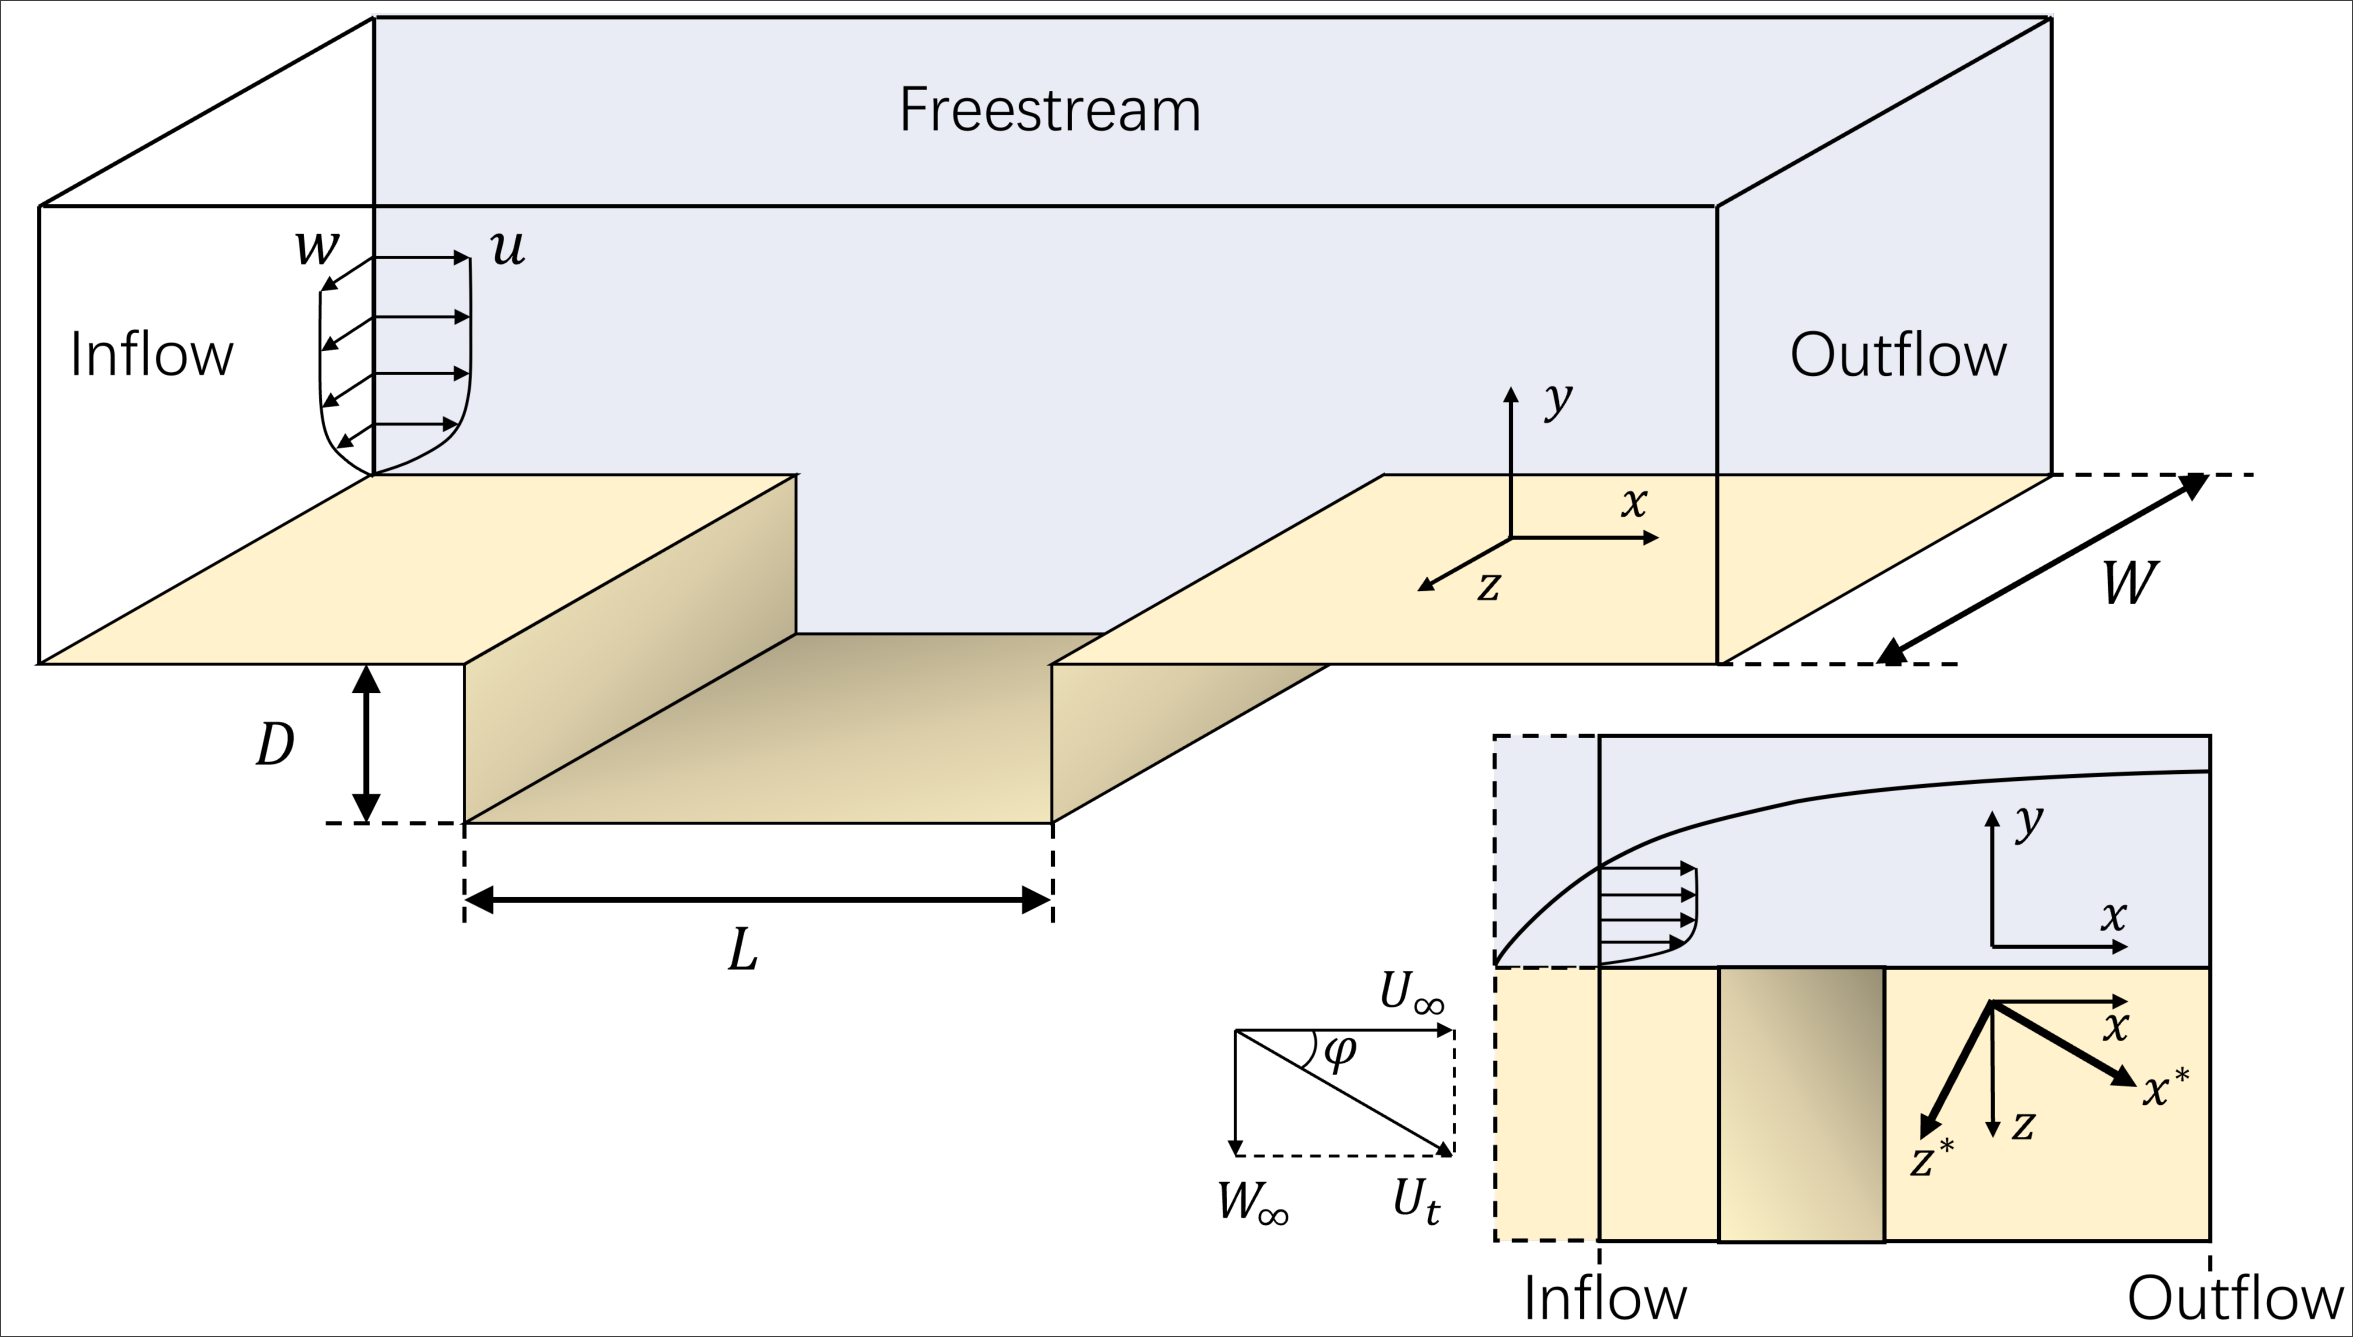
\includegraphics[trim=0.2cm 0.5cm 0.1cm 0.1cm, clip, width=\linewidth]{Images/domain.png} % Trimming is used to crop your image and the order of dimensions is: left, bottom, right, top. It's recommended to crop outside of LaTeX though, to ensure the aspect ratio remains the same.
			{\tiny\textcolor{ICLBlue}{From Ganlin's thesis}}
		\end{column}
	\end{columns}
\end{frame}

\begin{frame}
	\frametitle{Domain}

	\begin{columns}[T] % [T] ensures correct vertical alignment
		\begin{column}{0.28\linewidth} % Left column
			\textbf{Boundary conditions}
			\begin{itemize}
				\item Inlet \& outlet flows.
				\item Free stream at the top and no-slip at the bottom.
				\item Periodic in $z$ direction.

			\end{itemize}
		\end{column}
		\begin{column}{0.68\linewidth} % Right column
			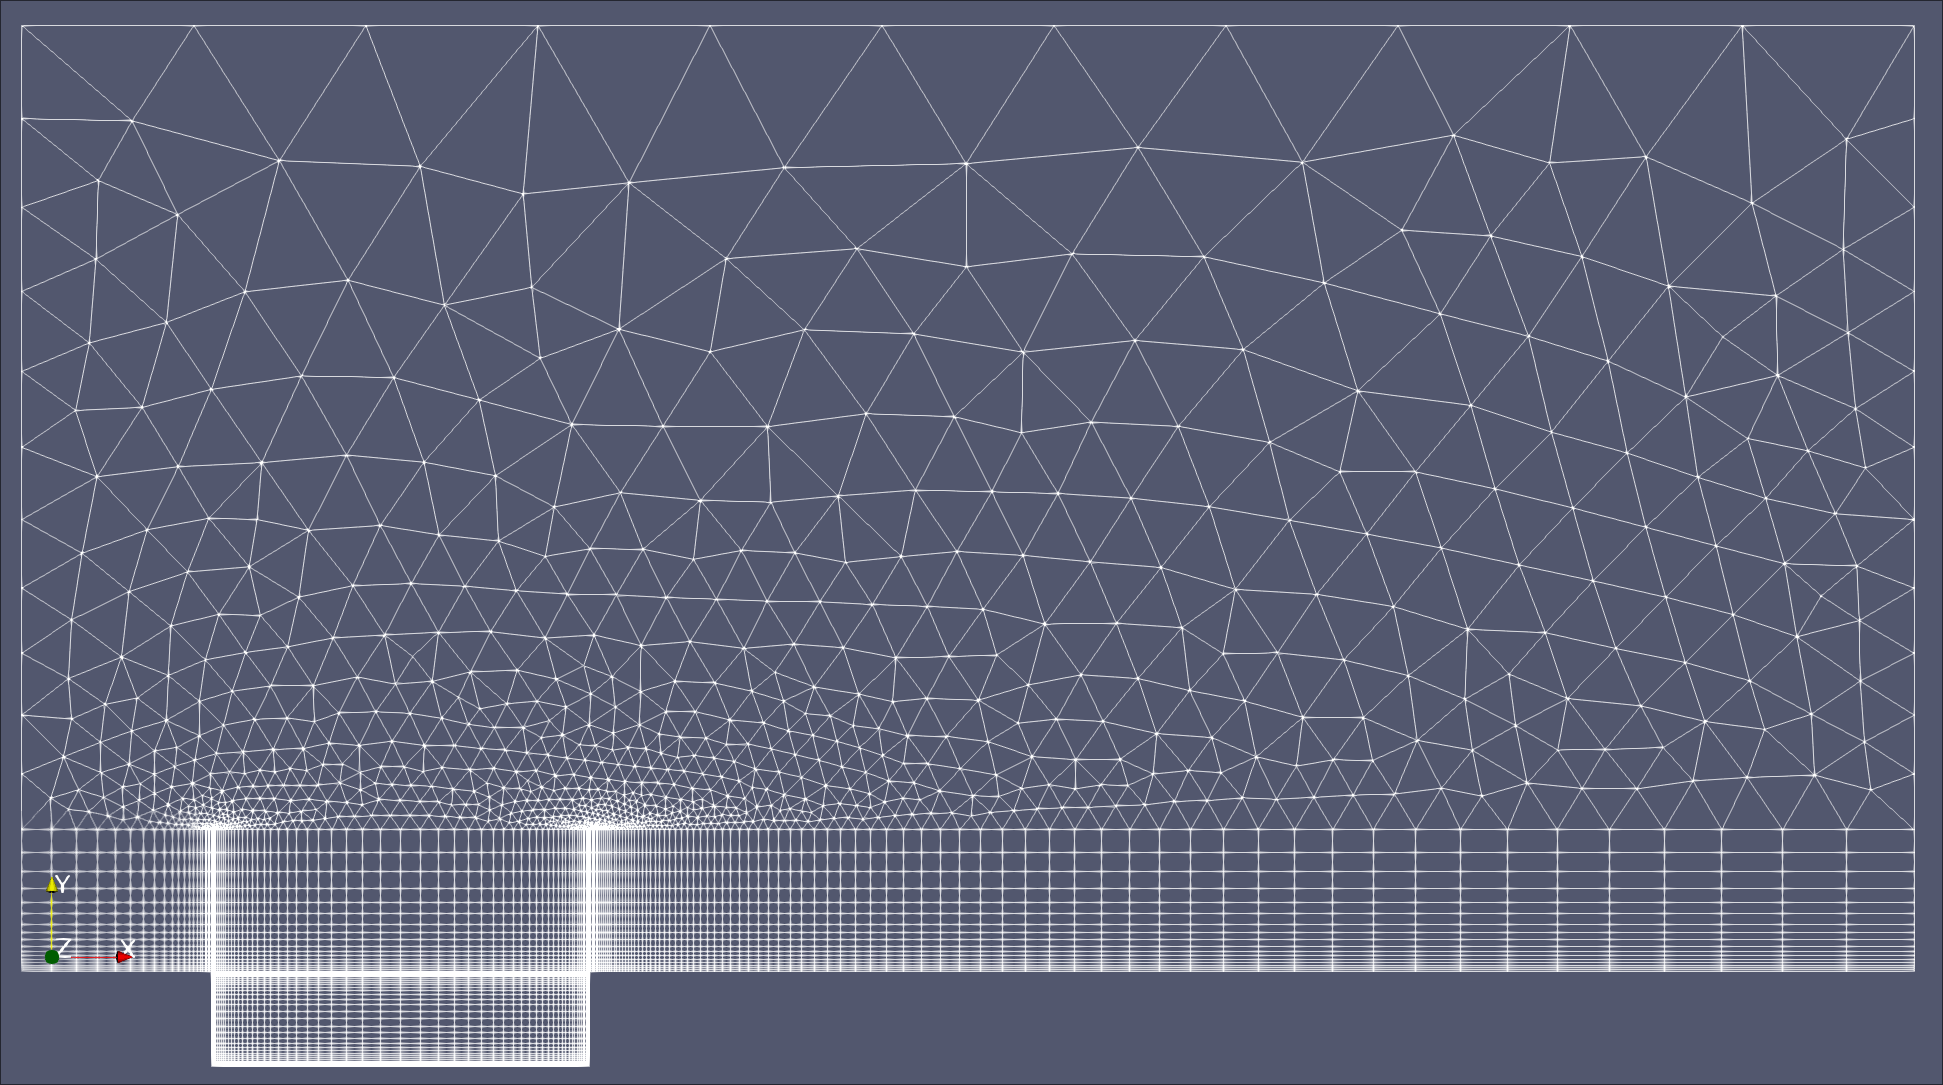
\includegraphics[width=\linewidth]{Images/mesh.png} % Trimming is used to crop your image and the order of dimensions is: left, bottom, right, top. It's recommended to crop outside of LaTeX though, to ensure the aspect ratio remains the same.
			{\tiny\textcolor{ICLBlue}{}}
		\end{column}
	\end{columns}
\end{frame}

\begin{frame}
	\begin{center}
    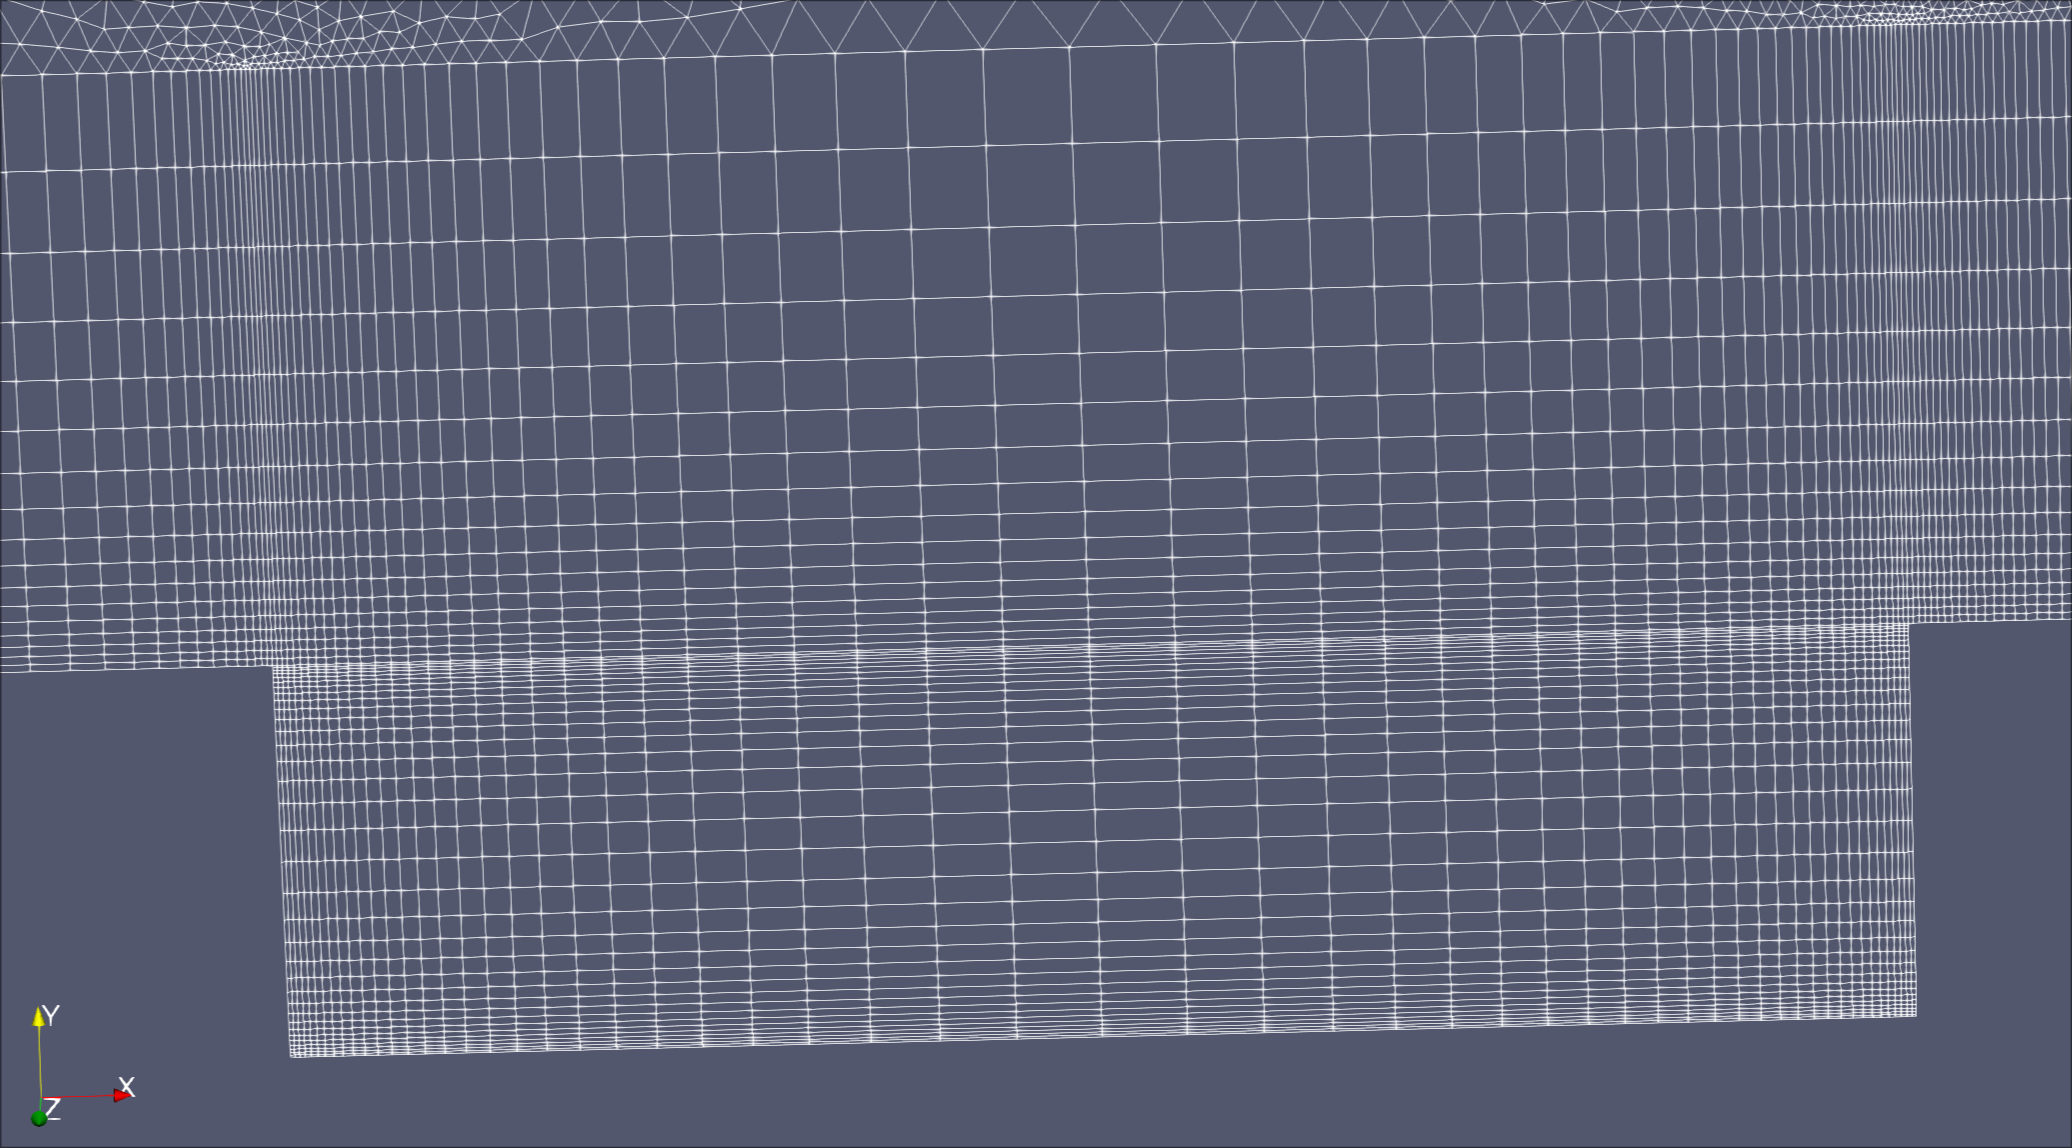
\includegraphics[width=0.7\linewidth]{Images/mesh_gap.png}
	\end{center}
	
\end{frame}

\begin{frame}
	\frametitle{Baseflow}

	\small % Reduce font size in this slide
	\begin{itemize}
		\item Quasi-3D simulations with 16 Fourier modes in the $z$ direction at $Re_D = 1500$ lead to a 2D stable baseflow (see pictures below).
		\item Quasi-3D simulations with only the constant mode in the $z$ direction at $Re_D = 7500$ lead to an unstable baseflow, which after using a feedback control in order to stabilize the problem, we get a baseflow similar to one the below.

	\end{itemize}
	\begin{columns}[T] % [T] ensures correct vertical alignment
		\begin{column}{0.3\linewidth} % Left column
			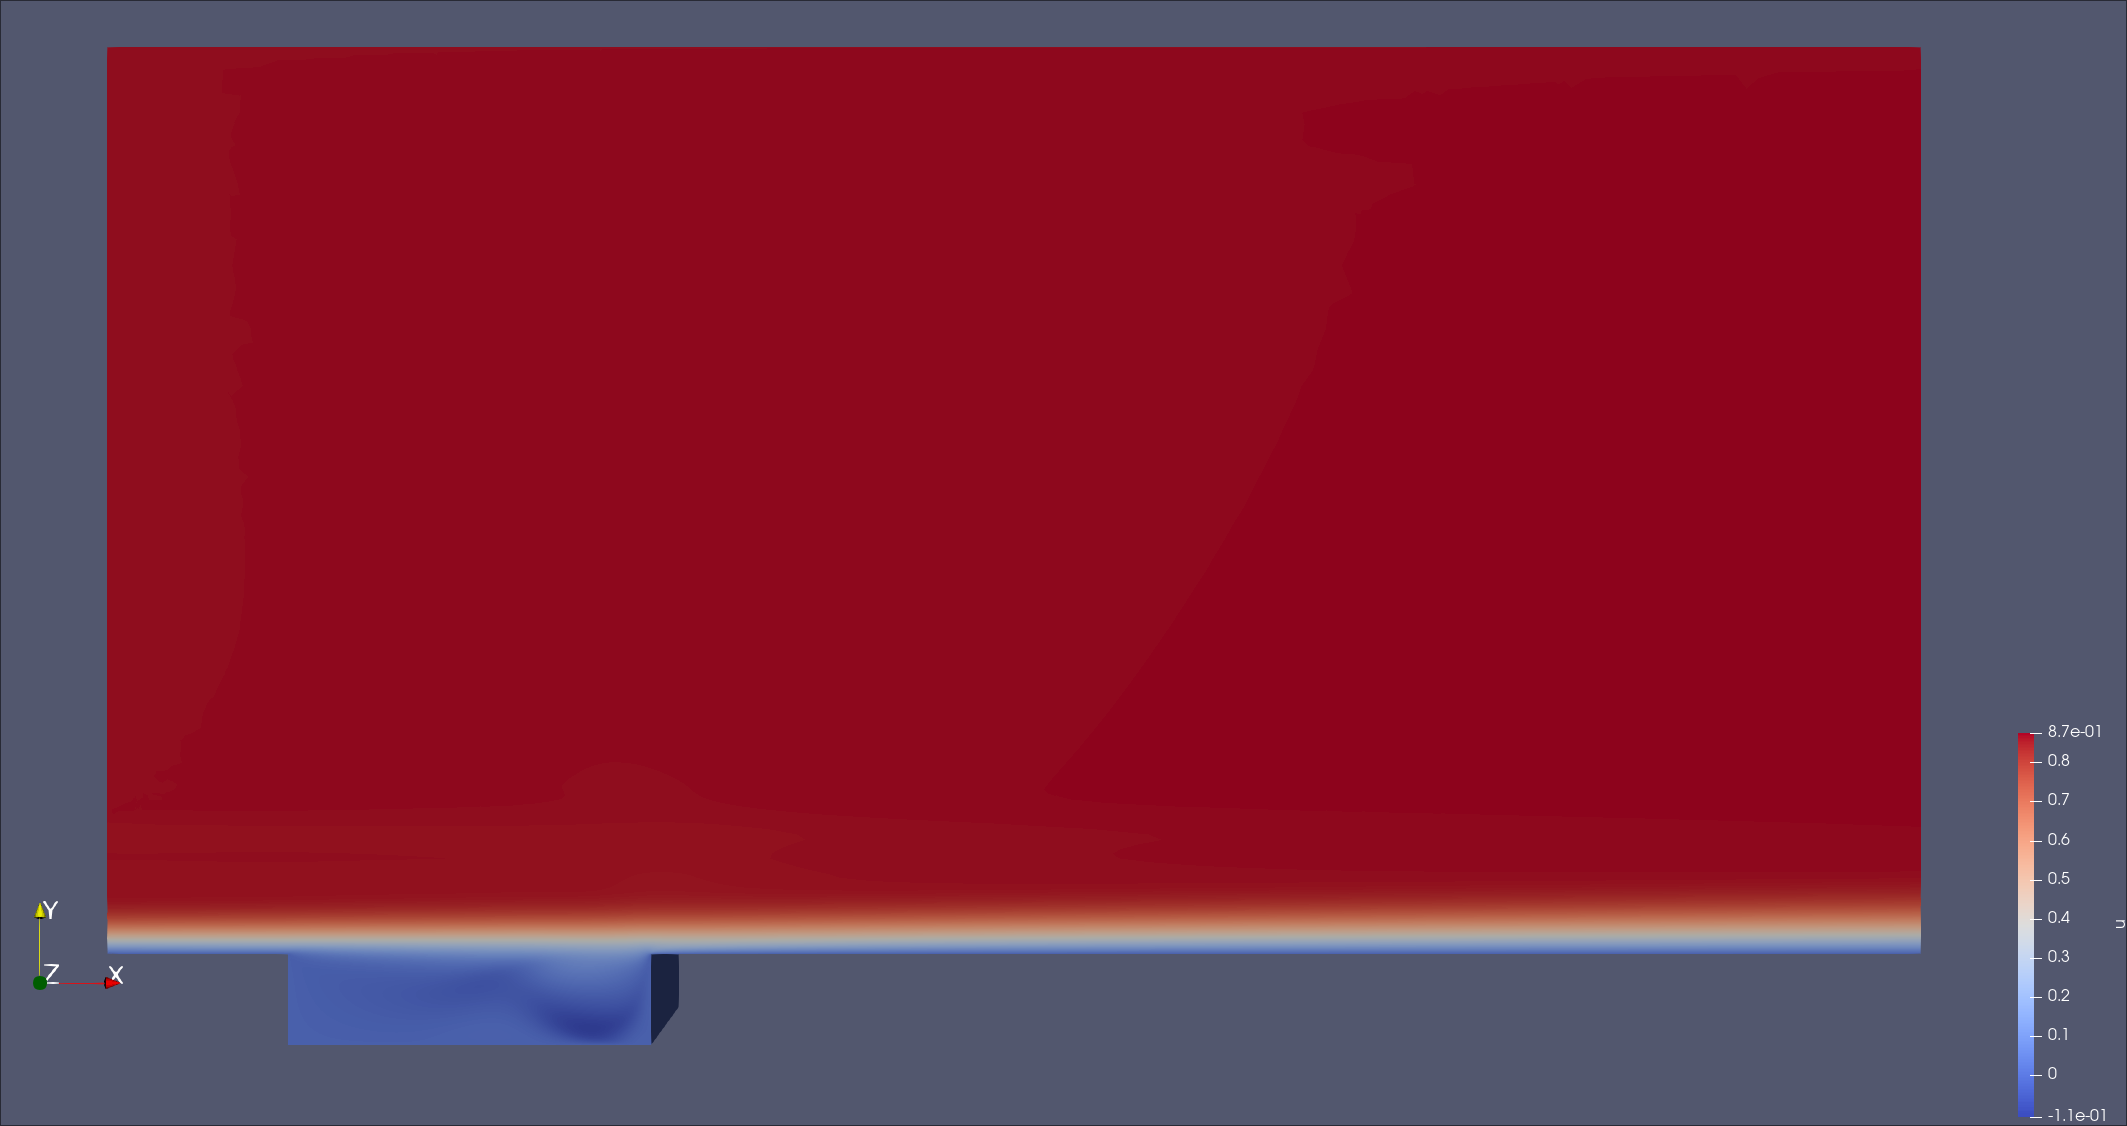
\includegraphics[width=\linewidth]{Images/baseflowU.png}\\[3pt]
			{\tiny\textcolor{ICLBlue}{$u$ component}}
		\end{column}
		\begin{column}{0.3\linewidth} % Center column
			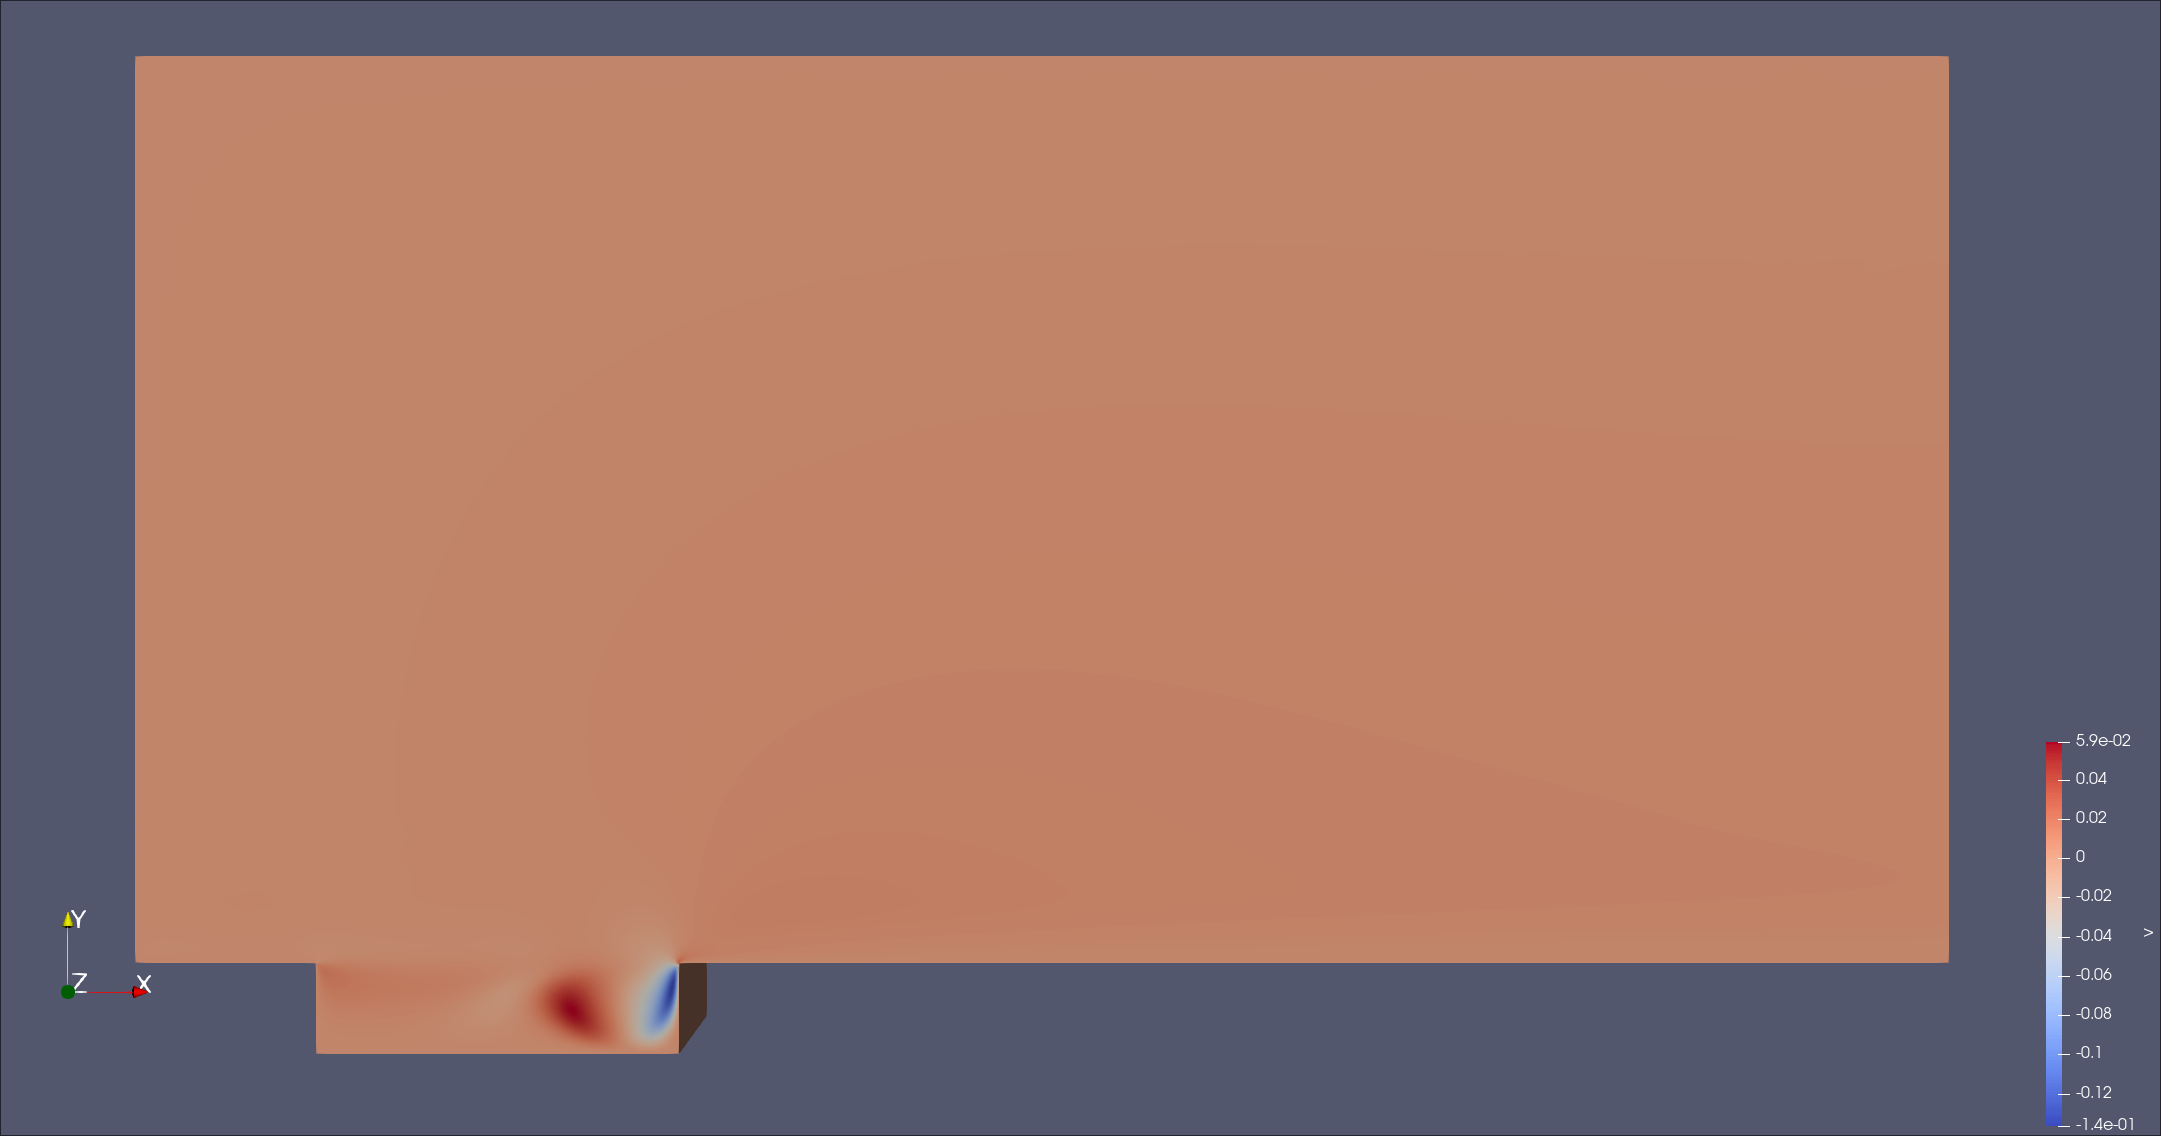
\includegraphics[width=\linewidth]{Images/baseflowV.png}\\[3pt]
			{\tiny\textcolor{ICLBlue}{$v$ component}}
		\end{column}
		\begin{column}{0.3\linewidth} % Right column
			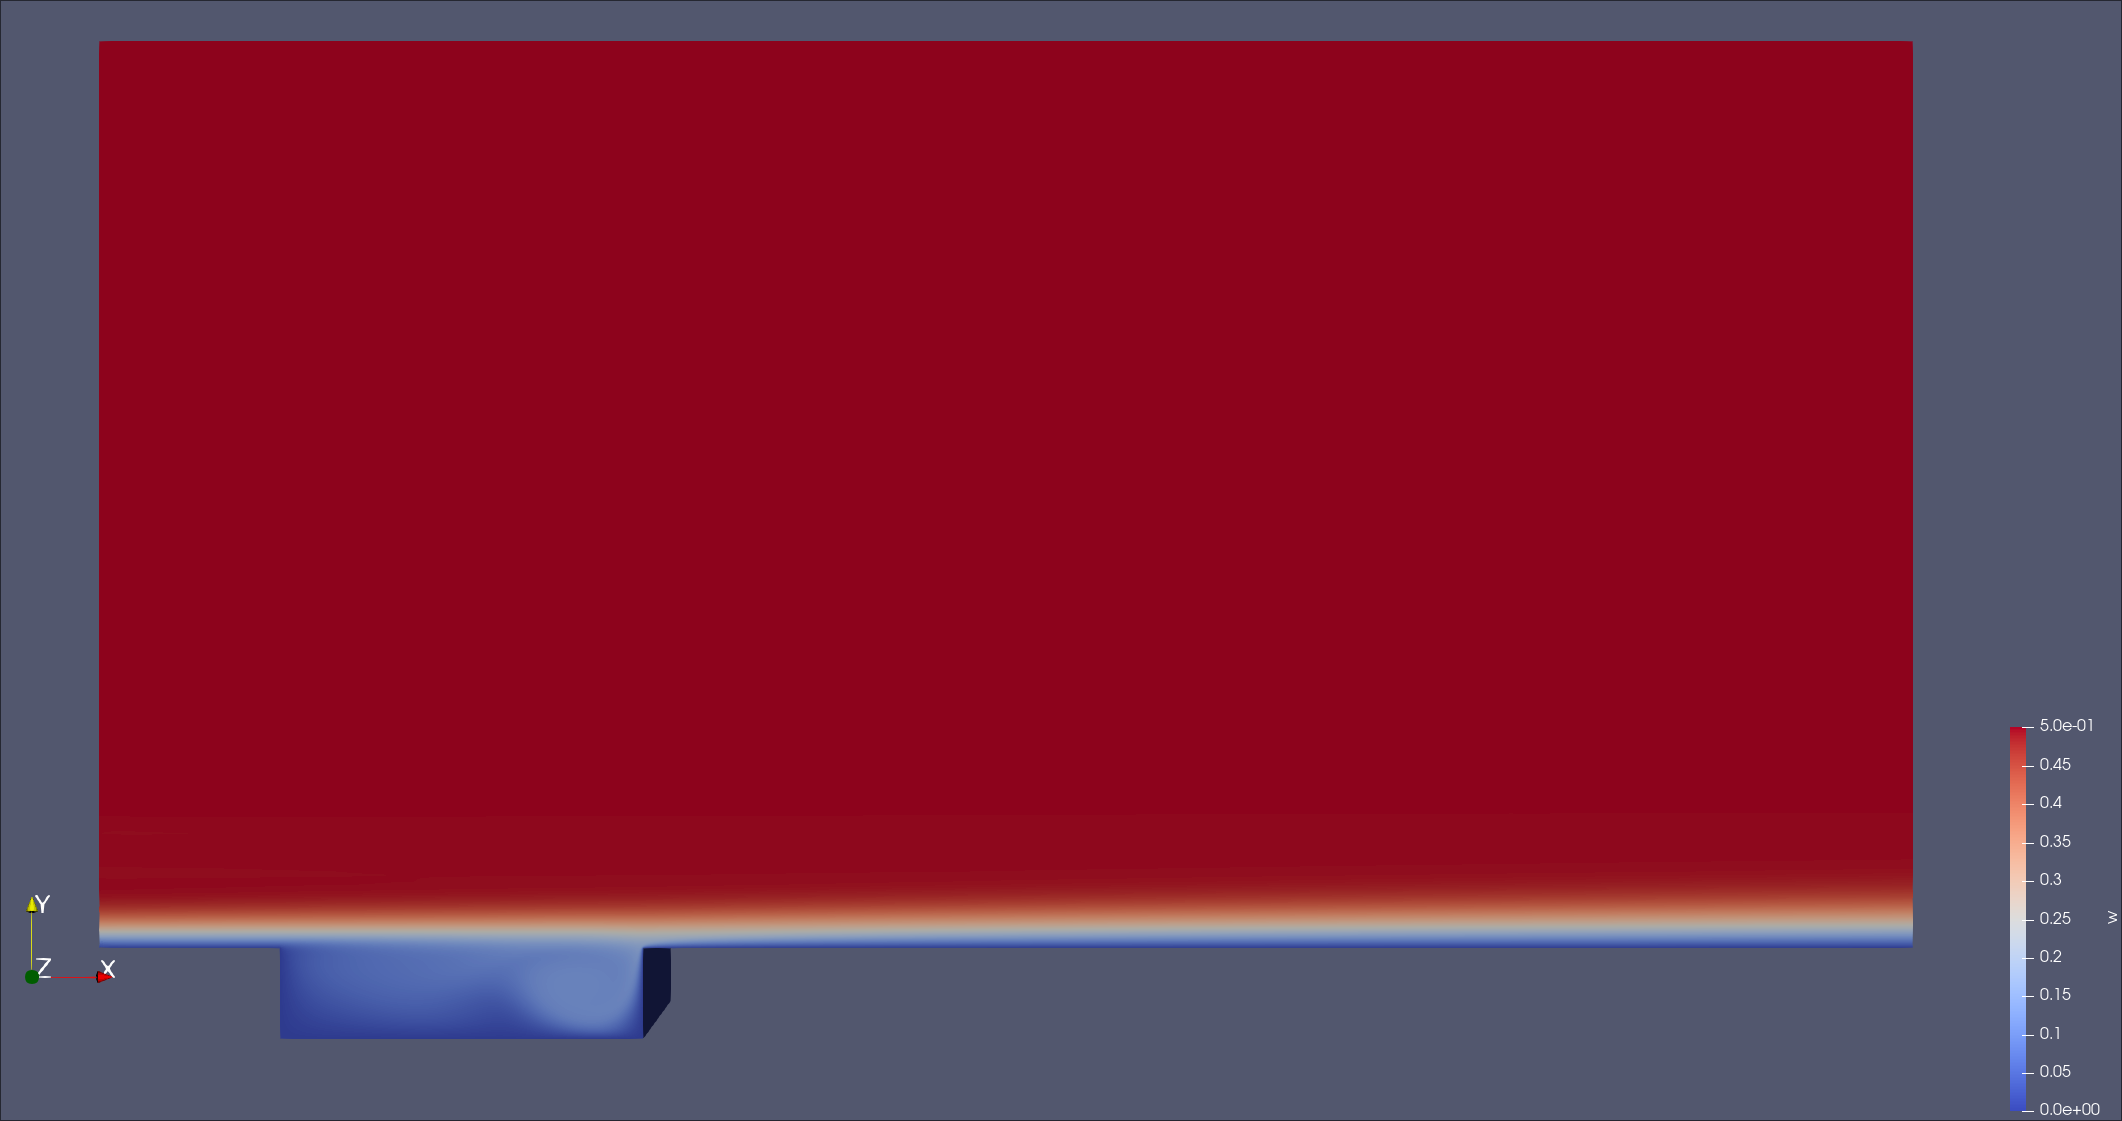
\includegraphics[width=\linewidth]{Images/baseflowW.png}\\[3pt]
			{\tiny\textcolor{ICLBlue}{$w$ component}}
		\end{column}
	\end{columns}
\end{frame}
\begin{frame}
	\frametitle{Preliminary LSA results ($Re_D = 7500$)}

	Single mode simulations by modifying the length of the domain in the $z$ direction. In each case we assume that the perturbation is of the form:
	$$
		\tilde{u}(x,y,z,t) = q(x,y) \exp(i\beta_n z) \exp(\lambda t)+c.c.
	$$
	where $\beta_n=2\pi n/L_z$ is the mode.
	We ran the linear Navier-Stokes for $n=1,\ldots,8$ in order to see which eigenpairs $(\lambda, q)$ are unstable.

	Modes 1, 2, 5, 6, 7 and 8 are stable.

	The leading eigenvalues of modes 3 and 4 have positive real part leading also to an instability.
\end{frame}

\begin{frame}

	\begin{center}
		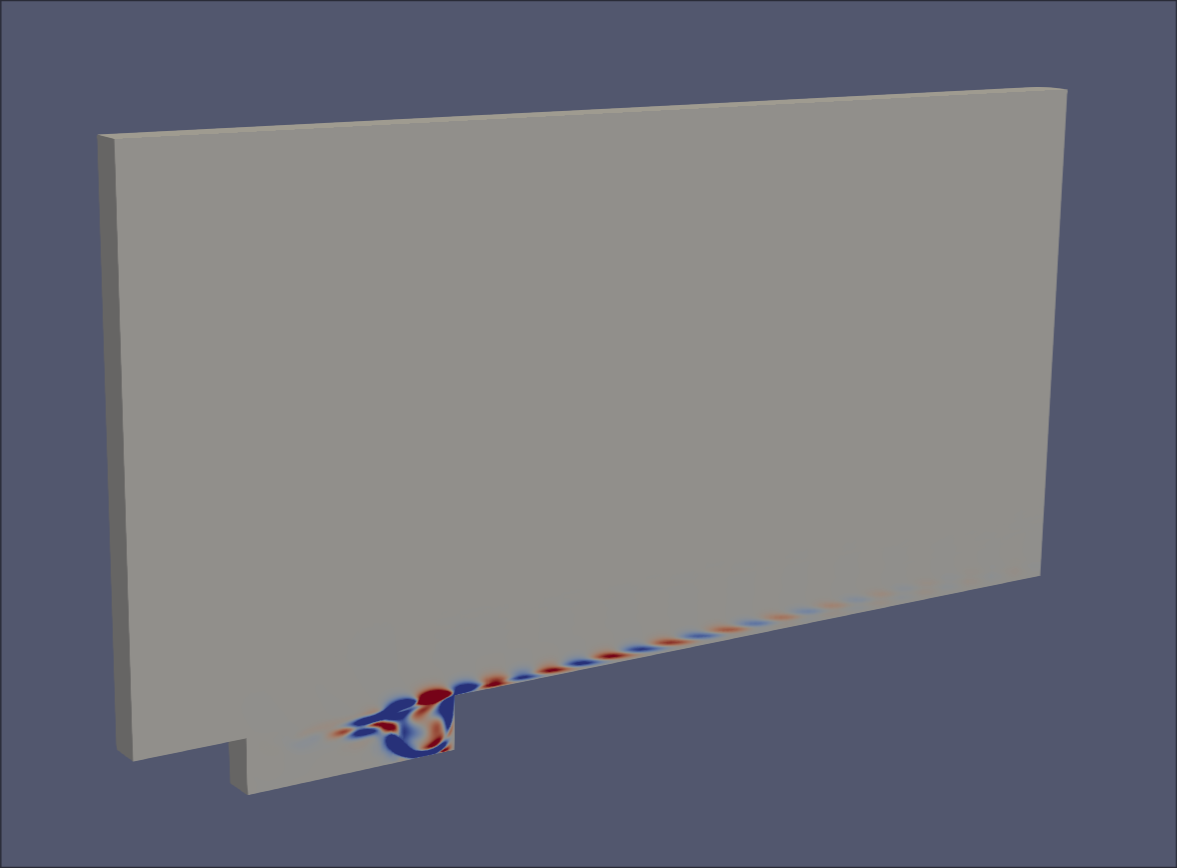
\includegraphics[width=0.5\linewidth]{Images/mode3_u.png}\\[3pt]
		{\tiny\textcolor{ICLBlue}{$u$ component of the velocity of an unstable mode with $\beta_3$}}
	\end{center}


	All the unstable modes that we plot so far look similar. Also $w$ component is \textit{similar} to $u$ component.
\end{frame}

\begin{frame}

	\begin{center}
		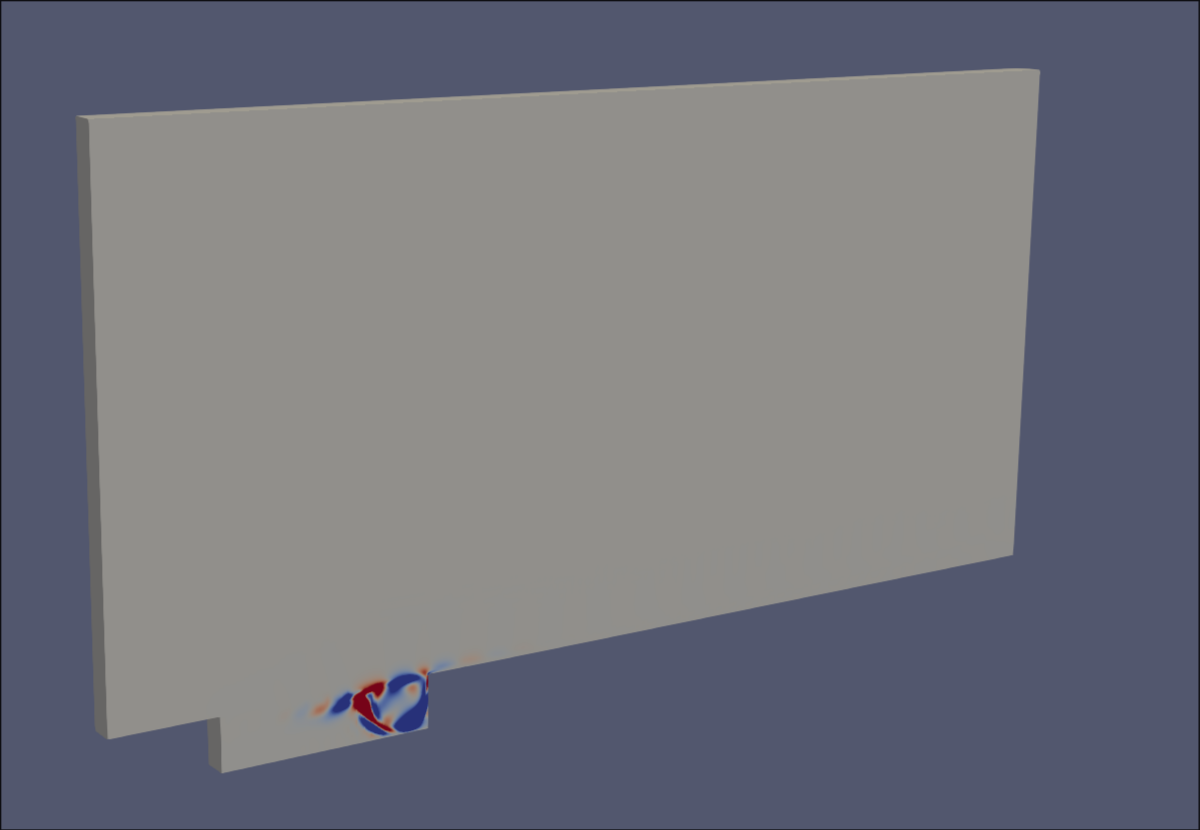
\includegraphics[width=0.6\linewidth]{Images/mode3_v.png}\\[3pt]
		{\tiny\textcolor{ICLBlue}{$v$ component of the velocity of the same unstable mode of above, with $\beta_3$}}
	\end{center}


\end{frame}

\begin{frame}

	\begin{center}
		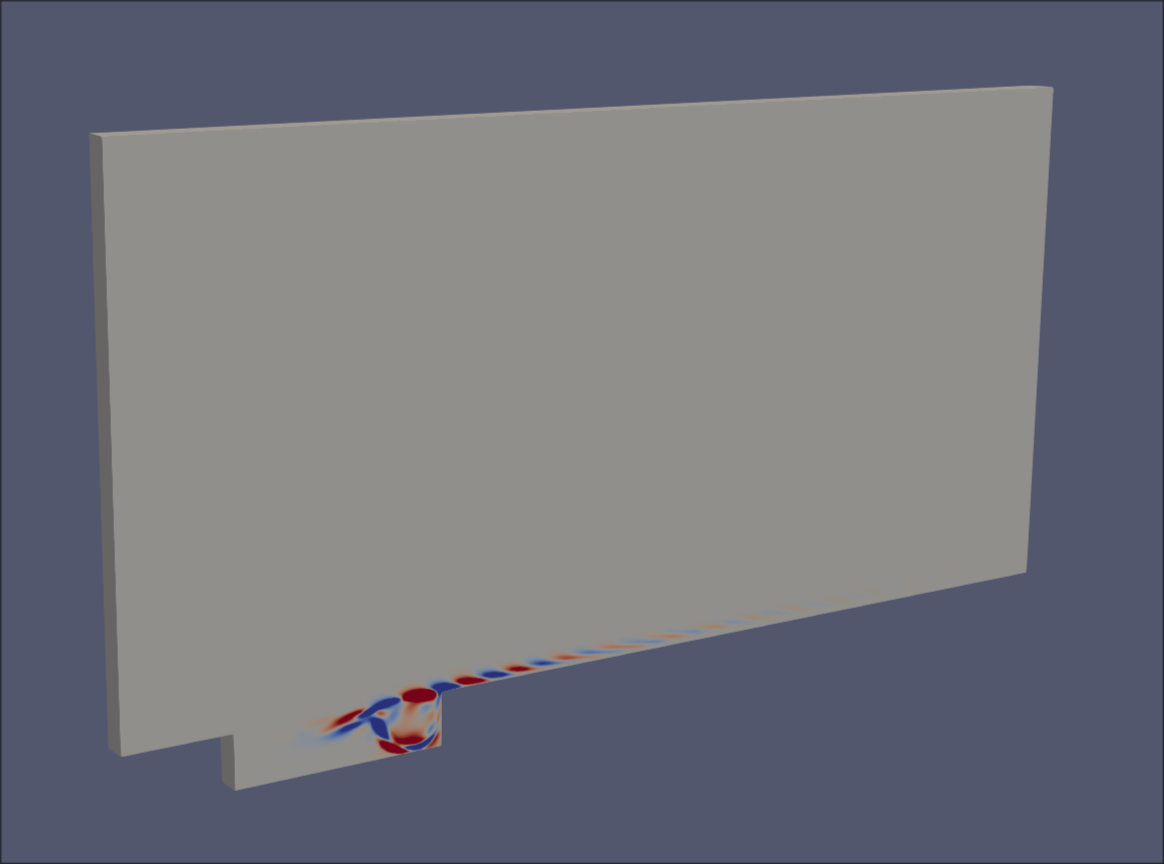
\includegraphics[width=0.6\linewidth]{Images/mode4_u.png}\\[3pt]
		{\tiny\textcolor{ICLBlue}{$u$ component of the velocity of an unstable mode with $\beta_4$}}
	\end{center}

\end{frame}

\begin{frame}
  \frametitle{Next steps, questions}

	\begin{itemize}
		\item How can we distinguish between convective instabilities within the gap and absolute instabilities? Because the domain is periodic in the $z$ direction, so a priori the latter ones may camouflage the former ones.
		\item Is the domain appropriate for Boeing's problem? Specific data is needed. Should we change the length ratios (1st slide)? In particular, the sweep angle may influence the appearance of certain unstable modes or not.
		\item Are we interested in the onset of the instabilities as a function of the Reynolds number?
		\item Should be start doing DNS simulations with the compressible solver?
	\end{itemize}
\end{frame}

\end{document}
